% Chapter where we explain the results.

\chapter{Discussion}
\label{ch:discussion}

In this section we provide justifications for the choices made in solving the
protoboard layout problem, and also detailed analysis of the data presented in
Chapter \ref{ch:results}.

\section{Justifying Placement Choices}
\label{sec:justify_placement}

\subsubsection{Resistors}

For the sake of simplicity, and to significantly reduce the search space
\q, for every resistor in the schematic, I use one resistor piece on the
protoboard placed in the middle strip of the protoboard as shown in Figure
\ref{fig:piece_placement}. This choice, i.e. allowing the resistor pieces to
only reside in the middle strip of the protoboard, is critical
as the resistor pieces can generally be placed at numerous places on the
protoboard.
With this restriction, there are $63$ slots available for one resistor. Without
this restriction, there are a total of $763$ slots available. The restirction is
good when we consider the reduction in the search space size. On the other hand,
the restriction is bad when we
consider the size of circuits the algorithm can layout. Given that the number
of resistors in a typical 6.01 circuit is very
small \q, this restriction proves to be very useful.

\subsubsection{Op Amps}

Op Amps are the trickiest components to handle because each Op Amp package put
on the protoboard contains two Op Amps within it. Equation
\ref{eq:opamp} presents an expression for the value $f(n)$, the number of
different ways to package together $n$ Op Amps. For example, if we have $2$ Op
Amps, we can either use one Op Amp package for each, or put them both in the
same package, which we can do in one of two different ways. Hence, $f(2) = 3$.
To get a sense of how many different packagings are possible, Table
\ref{tb:opamp} gives the values of $f(n)$ for various $n$.

\begin{equation}
f(n) = \sum\limits_{k=0}^{\lfloor\frac{n}{2}\rfloor}{\frac{n!}{k!(n - 2k)!}}
\label{eq:opamp}
\end{equation}

\begin{table}
\begin{center}
\begin{singlespace}
\begin{tabular}{c | c}
$n$ & $f(n)$ \\
\hline
\hline
1 & 1 \\
2 & 3 \\
3 & 7 \\
4 & 25 \\
5 & 81 \\
6 & 331 \\
7 & 1303 \\
8 & 5937 \\
9 & 26785 \\
10 & 133651
\end{tabular}
\end{singlespace}
\end{center}
\label{tb:opamp}
\caption{Number of ways of packaging together $n$ Op Amps for various values of
$n$.}
\end{table}

Our placement approach explores all possible ways
of packaging up the Op Amps. We do this because the typical 6.01 circuit contains
no more than $6$ Op Amps, and so we are tasked with exploring at most $331$
alternatives, which doesn't happen to be too computationally intensive. If the
algorithm was meant to handle a larger number of Op Amps (for example $10$), then
this approach would be silly, and we would have to resort to perhaps considering
the packagings that require the fewest number of Op Amps to make a choice.

\subsubsection{Pots}

Each pot piece can be placed in one of two vertical locations on the protoboard.
Each pot piece also has two possible orientations. TODO: really 6 different
vertical locations.

\subsubsection{Head, Motor, and Robot Connectors}

Our choices for the connector pieces is certainly one of the two presented in
Figure \ref{fig:piece_placement}. Any other placement of the connector pieces
would unecessarily take up valueable rows.

\section{Explaining the Results}

Chapter \ref{ch:results} presented quantitative data to compare the various
alternatives we have in solving the protoboard layout problem. Here, we will
analyze that data and give reasonings for why we obtained the results
that we obtained. For each comparison, we present exemplar layouts generated
by the alternative methods for the schematic shown in Figure
\ref{fig:exemplar_schematic}.

\begin{figure}
\begin{center}
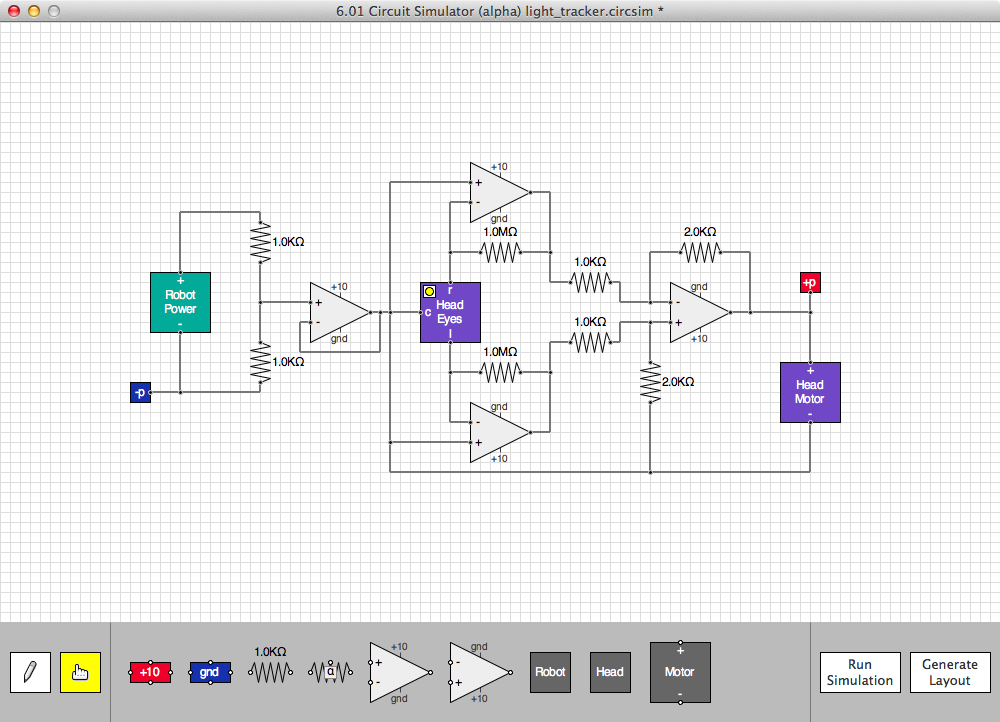
\includegraphics[width=\textwidth]{Images/exemplar_schematic.png}
\caption{Exemplar schematic.}
\label{fig:exemplar_schematic}
\end{center}
\end{figure}

\subsection{Comparing placement methods}

In Figure \ref{fig:placement_success} and Table \ref{tb:placement_success} we
see that the distance method exceeds the blocking method in number of circuits
solved $10$ times out of $10$ as well as in the number of circuits solved $0$
to $2$ times out of $10$. On the other hand, the blocking method exceeds the
distance method in number of circuits solved from $3$ to $9$ times out
of $10$. Overall, the blocking placement method is slightly more successful
than the distance placement method. Despite this difference, we note that the
two alternatives have very
close success rates. As a function of circuit complexity, Figure
\ref{fig:placement_success_trend} suggests that the two alternatives have almost
identical success rates. As we would expect, we certainly observe that as the
complexity of the circuits
increases, success rate generally decreases for both of the placement methods.
The curves in Figure \ref{fig:placement_success_trend} seem to shoot back up
at the far end of the figure, but this is a result of the fact that there are
very few circuits at that end of the figure, on which the algorithm happened to
be consistently successful.

When we consider wiring time as the basis for comparison, we observe from
Figure \ref{fig:placement_time_trend} that, once again, the two metods are
very similar. We see that the distance method generally takes slightly less
wiring time than the blocking method, but the difference between the two is
almost negligible. As we would expect, we certainly see that as the complexity
of the circuits increases, the amount of time spent by the wiring step also
increases. As we did for the success rate trends as a function of circuit
complexity, we observe that there are outliers at the far end of the figure due
to a very small sample of the most complex circuits in the randomly generated
schematic dataset.

Finally, let us look at layout complexity as the basis for comparison. Figure
\ref{fig:placement_quality_trend} presents graphs that compare numbers of wires,
numbers of wire crosses, and total wire lengths. We first observe that the
number of wires used by the two methods are almost identical. As the complexity
of the circuit increases, we see that the blocking method uses more wires than
does the distance method, but by and large the values are very comparable. This
makes intuitive sense as we are rarely required to use more wires than
absolutely necessary (keeping wires horizontal and vertical) to connect a pair
of locations (?). When we look at the number of wire crosses in the layouts, we
see that the blocking method consistently results in more wire crosses. Similarly,
when we look at the total length of wires used in the layouts, the blocking
method exceeds the distance method consistently, with the difference getting
higher as complexity increases. This can be explained by the fact that the
blocking method may require elaborate connections, especially as the circuits
get more complex while the distance method is tuned to require wirings between
pairs of locations that are closer together.

It is difficult to conclusively pick the better placement method from these results.
It is clear that both methods have their strengths and weaknesses. In Section
\ref{sec:method_combination} we will discuss how combining these two methods can
get us the best of both worlds (?).

\begin{figure}
\begin{center}
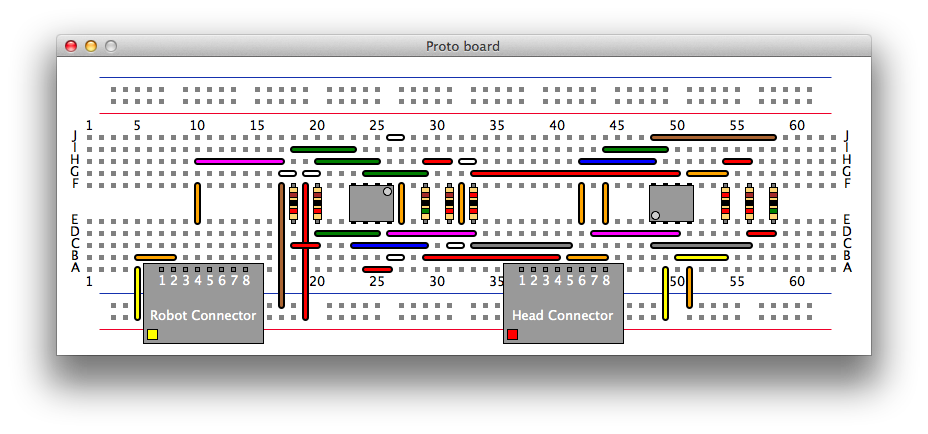
\includegraphics[width=\textwidth]{Images/exemplar_per_pair_decreasing.png}
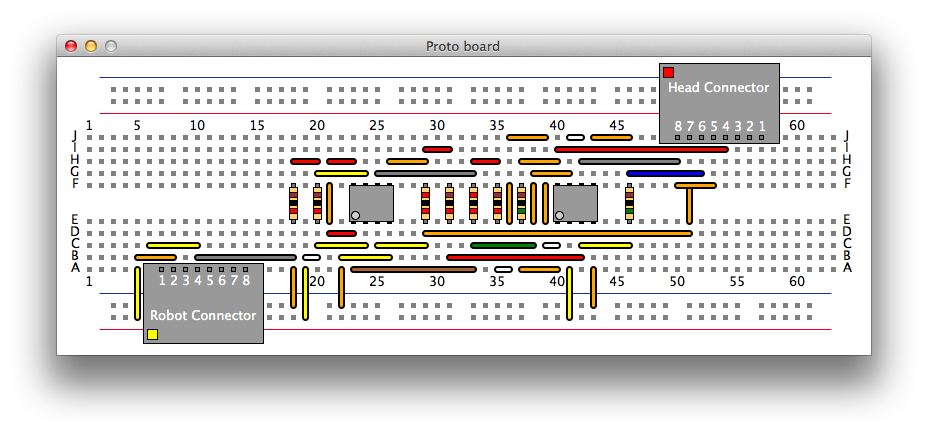
\includegraphics[width=\textwidth]{Images/exemplar_distance.png}
\caption{Blocking vs. Distance.}
\end{center}
\end{figure}

\subsection{Comparing wiring methods}

To compare the wiring methods, let us start with the success rate for each method.
Figures \ref{fig:wiring_success} and \ref{fig:wiring_success_trend}, and Table
\ref{fig:wiring_success} provide the appropriate data. The very first fact we
observe is that the all-pairs method has a much smaller success rate than all of
the other alternatives, especially as circuit complexity increases. The reason
for this, in large part, is the fact that we impose a cutoff on the number of
nodes to expand in the search (TODO: this must be discussed in Methods). As we
are using just the one search to connect all pairs of locations, the search
cutoff would be expected to have more of an effect on the all-pairs method. The
other four alternatives have very comparable success rates.

Next we look at Figure \ref{fig:wiring_time_trend} to compare wiring times for
the five methods. Once again, we observe that the all-pairs methods takes
significanlty more time than the other methods. When attempting to connect all
pairs in one search, the method searches for an appealing layout, which may
require searching through a large number of alternatives, especially for more
complex circuits. Hence, we would expect the all-pairs methods to generally take
more time than the other alternatives. We also observe from Figure
\ref{fig:wiring_time_trend} that the wiring times for the two per-node methods
are comparable, and that the wiring times for the two per-pair methods are also
comparable, but that the per-node wiring times are generally bigger than the
per-pair wiring times. This trend is also expected as the per-node methods
attempt to connect multiple pairs of locations at once while keeping the layout
pleasing, and this generally requires searching through more alternatives than
connecting each of the pairs of locations individually. It is important to note
that per-node, increaseing generally takes more time than per-pair, decreasing,
and also that per-pair, increasing generally takes more time than per-pair,
decreasing.

Finally let us look at Figure \ref{fig:wiring_quality_trend} to compare the
quality of the layouts produced by the five alternative wiring methods. First,
as we observed in the placement method comparison, we see that there is very
little difference in terms of number of wires used and the total wire length.
However, there are significant differences in the number of wire crosses. We see
that the all-pairs method generates layouts with much fewer wire crosses than
the other methods. This is completely expected since we run one search to
connect all pairs of locations while attempting to keep the layout as nice as
possible. Conversely, the per-pair, decreasing and per-node, decreasing methods
result in the most number of wire crosses. It is very interesting to note that
the per-node, decreasing method produces more wire crosses on average than the
per-pair,
increasing method. Here we observe that the order in which we consider pairs of
locations has a telling effect on how good the layouts will be. In essence,
connecting the harder pairs of locations generally produces more wire corsses.

What we have observed is that while the all-pairs method is the least successful
method and the one that generally takes the longest among the five,
it generally produces the best layouts when it does succeed. On the other hand,
the alternatives that break down the problem into smaller pieces succeed more
often and finish more quickly while producing worse results. Furthermore,
the more finely we breakdown the problem, the faster the overall algorithm.
Lastly, ordering subproblems from hardest to easiest has the effect of making the
overall wiring step complete faster but producing worse results than the reverse
order and not necessarily getting a markedly better success rate.

\begin{figure}
\begin{center}
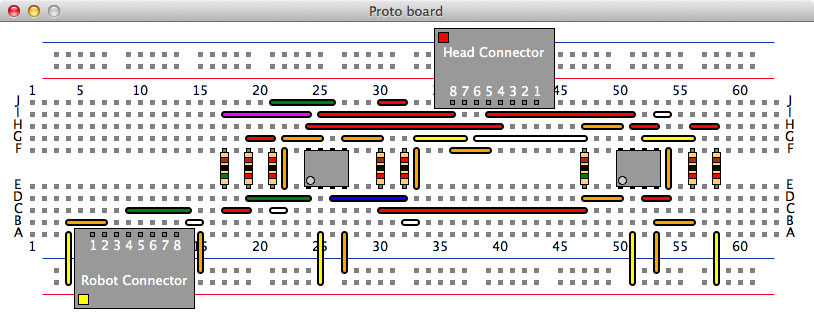
\includegraphics[width=\textwidth]{Images/exemplar_all_pairs.png}
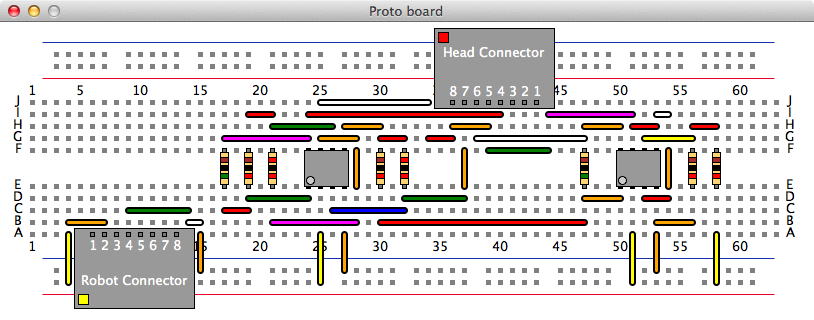
\includegraphics[width=\textwidth]{Images/exemplar_per_node_increasing.png}
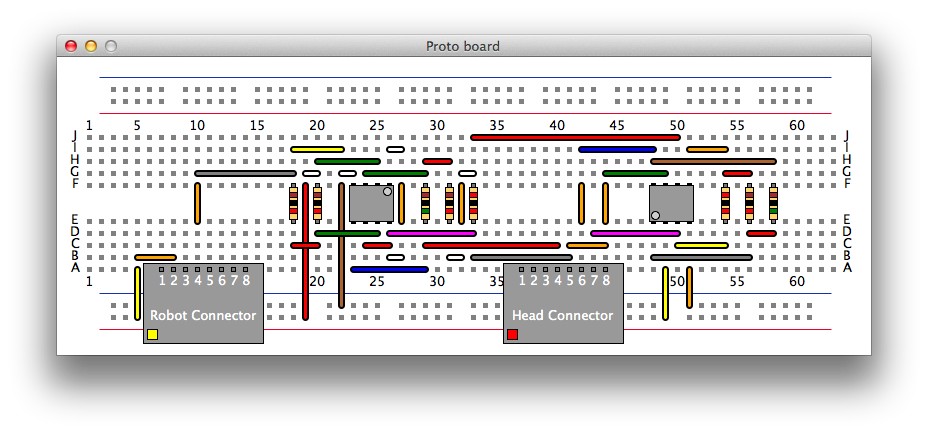
\includegraphics[width=\textwidth]{Images/exemplar_per_node_decreasing.png}
\end{center}
\end{figure}
\begin{figure}
\begin{center}
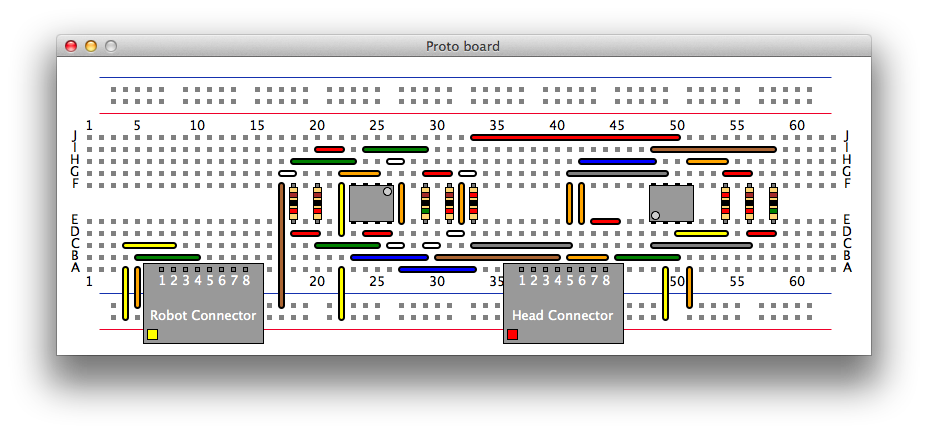
\includegraphics[width=\textwidth]{Images/exemplar_per_pair_increasing.png}
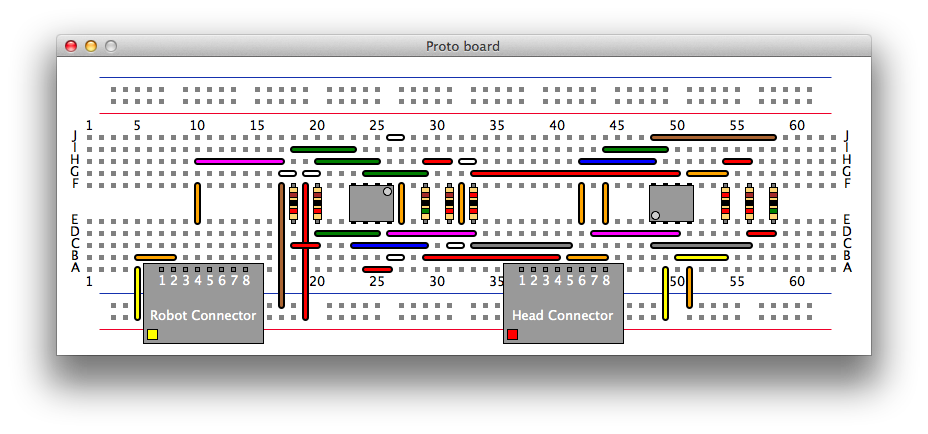
\includegraphics[width=\textwidth]{Images/exemplar_per_pair_decreasing.png}
\caption{All-pairs vs. Per-node, increasing vs. Per-node, decreasing vs.
Per-pair, increasing vs. Per-pair, decreasing.}
\end{center}
\end{figure}

\subsection{Comparing resistor treatments}

We now look at the two alternative treatments for wires: as components vs. as
wires. From Figures \ref{fig:resistor_success} and \ref{fig:resistor_success_trend}
and Table \ref{tb:resistor_success}, we observe that treating resistors as wires
results in a considerably smaller success rate than treating resistors as
components. Recall that the wiring method used here is per-pair, decreasing wiring.
When treating resistors as wires, we get more location pairs to connect.
The key difference for
the location pairs that correspond to resistors is that in connecting the given
pair of locations with wires, one of the wires is required to have length $3$,
the length of a resistor. Intuitively, this restriction should make the search
harder, and the data we have obtained suggests that the search is indeed
significantly more difficult with the restriction than without.

When we treat resistors as wires, and the search does succeed, we observe from
Figure \ref{fig:resistor_time_trend} that it takes more time than treating
resistors as wires, as expected.

Finally we look at the quality of layouts produced by the two methods. First,
we observe from Figure \ref{fig:resistor_quality_trend} that treating resistors
as wires produces layouts with fewer wires and smaller total length of wires
than treating resistors as components. This is certainly expected because each
resistor can be suitably placed to require fewer wires than would be required
if we forced the resistor to reside in the middle strip of the protoboard. We
do note, however, that treating resistors as wires results in more wire crosses
despite requiring fewer wires, especially as circuit complexity increases. This
can be attributed to the fact that treating resistors as wires is likely to
produce more compact layouts in which wire crosses are more likely to happen
than the spreadout settings we force when we treat resistors as components.

In this comparison, we can easily state that, with a limited search (i.e. with
a search in which we have a limited number of states to expand), treating
resistors as components is a better strategy than treating resistors as wires
based on the big difference in success rate.

\begin{figure}
\begin{center}
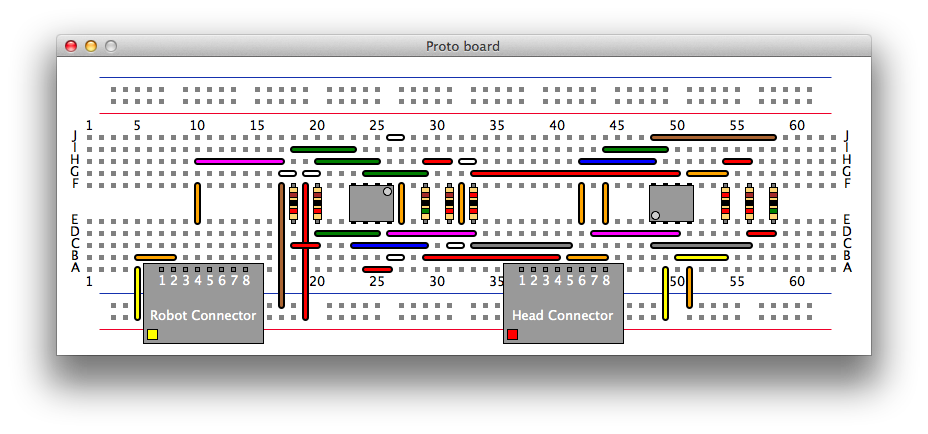
\includegraphics[width=\textwidth]{Images/exemplar_per_pair_decreasing.png}
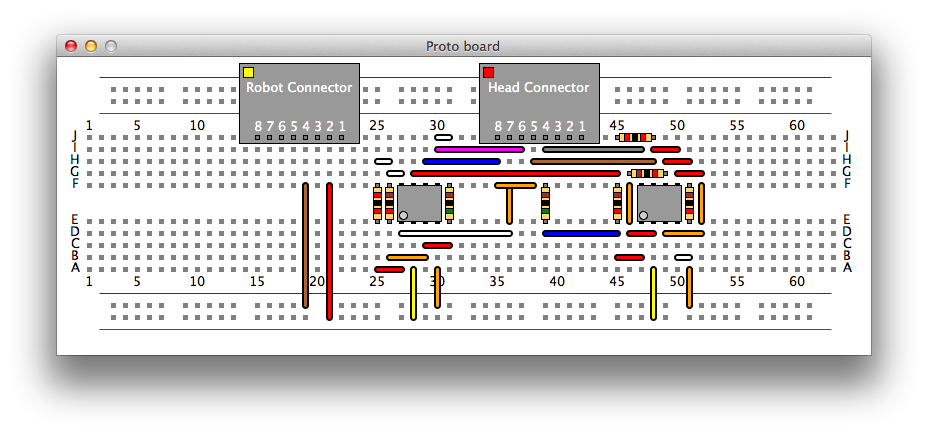
\includegraphics[width=\textwidth]{Images/exemplar_resistors_as_wires.png}
\caption{Resistors as components vs. Resistors as wires.}
\end{center}
\end{figure}

\subsection{Comparing search methods}

We now compare our two alternative search algorithms: $A*$ and Best First Search.
Let us start by comparing success rates. Figures \ref{fig:search_success} and
\ref{fig:search_success_trend} and Table \ref{fig:search_success} present the
appropriate data. We clearly observe that Best First Search is much more
successful than $A*$. $98\%$ of the test circuits were solved at least $8$ times
out of $10$ when we used Best First Search, versues $85\%$ when we used $A*$.
This result is not surprising because Best First Search hungrily hunts for
layouts that satisfy the connection requirements without caring for the
aesthetics of the layouts. Hence, Best First Search is much less succeptible to
the $300$ states to expand restriction than $A*$. The fact that the quality of
the results we get from Best First Search are worse
is clearly evident from Figure \ref{fig:search_quality_trend}. Most importantly, the
number of wire crosses in the layouts produced by Best First Search are markedly
greater than the number of wire crosses in the layouts produced by $A*$. We also
observe that the total wire length is greater when using Best First Search. The
fact that Best First Search settles for any layout that satisfies the connection
requirements suggests that it should finish more quickly in addition to being
more successful. Firgure \ref{fig:search_time_trend} supports exactly this
expectation.

Our choice of a search algorithm forces us to consider a treadoff between quick
success and quality. If we choose Best First Search, most runs will be successful
and terminate quickly, but will produce very poor results. If we choose $A*$,
not as many runs will be successful, and the successful runs will take longer to
terminate, but we will get much better layouts.

\begin{figure}
\begin{center}
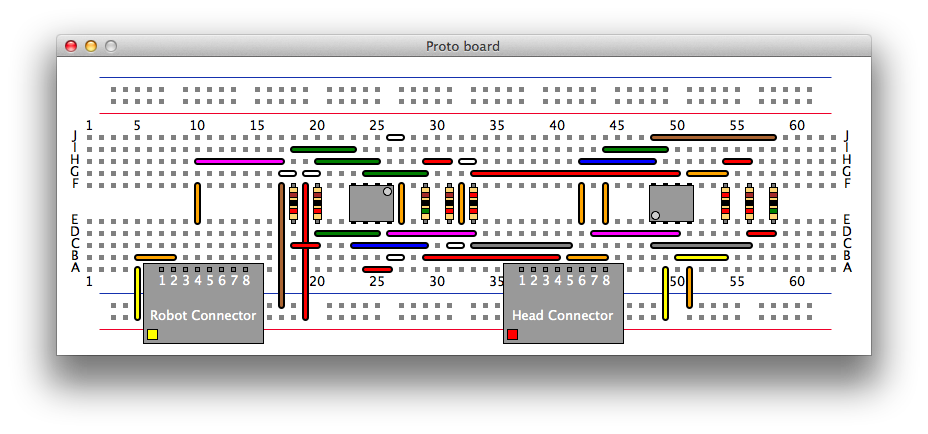
\includegraphics[width=\textwidth]{Images/exemplar_per_pair_decreasing.png}
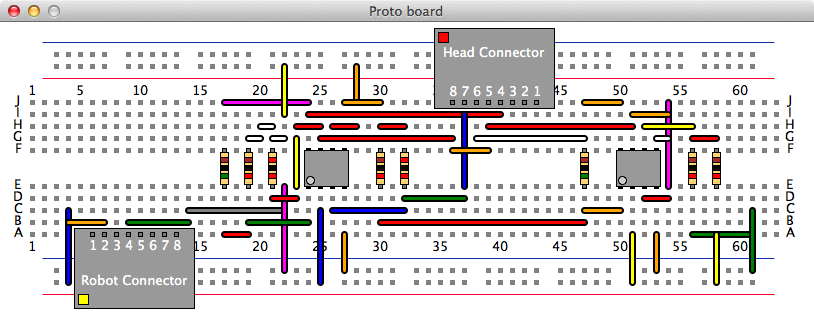
\includegraphics[width=\textwidth]{Images/exemplar_best_first.png}
\caption{$A*$ vs. Best First Search.}
\end{center}
\end{figure}

\subsection{Putting them all together}
\label{sec:method_combination}

\section{Remarks}

\textit{Why are these results encouraging? What are their implications? Relate
back to Introduction to Thesis. What could have been done differently?}
